
\documentclass[a4paper, 10pt]{IEEEconf}  

\usepackage{geometry}
\geometry{a4paper, margin=1in}
  
  
\usepackage{subcaption}  
\usepackage[export]{adjustbox}    
\usepackage{verbatim}
\usepackage{graphicx}
\usepackage{pdfpages}
\usepackage{cite}
\usepackage{listings}
\usepackage{float}
\usepackage{url}
\usepackage{hyperref}
\usepackage{fancyhdr}
\usepackage{multicol}

\lstset{
	tabsize=2,
	breaklines=true
}

\setlength{\parskip}{1em}
\onecolumn

\title{\LARGE \bf Assignment 1: Mobile Robot ROS Gazebo\\Simulation Modelling and Optimisation 282 758}
\author{Marc Alexander Sferrazza \\ 12164165
\thanks{This work was not supported by any organization}
\thanks{Faculty of Mechatronics Engineering, Massey University, Albany, Auckland, New Zealand
        {\tt\small Progress of project: https://github.com/alex1v1a/Simulation-Modelling-and-Optimisation/} } }

\begin{document}

\maketitle
\begin{figure}[h]
\begin{subfigure}{0.5\textwidth}

\includegraphics[width=1.5\textwidth, left]{images/ROS} 
%\caption{ROS}
\label{fig:ROS}
\end{subfigure}
\begin{subfigure}{0.5\textwidth}

\includegraphics[width=0.3\textwidth, right]{images/gazebo}
%\caption{Gazebo} 
\label{fig:Gazebo}
\end{subfigure}
%\caption{Caption for this figure with two images}
%\label{fig:image2}
\end{figure}
\begin{figure}[H]
  \begin{center}
  
\includegraphics[width=110mm]{images/kinetic}
  \label{fig:kinetic}
  \end{center}
\end{figure}
\thispagestyle{empty}
\pagestyle{plain}


%%%%%%%%%%%%%%%%%%%%%%%%%%%%%%%%%%%%%%%%%%%%%%%%%%%%%%%%%%%%%%%%%%%%%%%%%%%%%%%%

%\begin{abstract}

%In this assignment you will setup ROS on your computer and install Gazebo simulator. ROS has a number of robot models ready for using in Gazebo, of which you can choose one and link it to main ROS packages for tele-operation from your keyboard. Add a laser scanner (e.g. Hokuyo URG or Sick Scanner) to the robot making sure the scanner publishes laser data over ROS. One choice of the robot model could be Poineer-3DX which is also available in hardware form. Your simulated code will run on the real robot without modification. 

%\end{abstract}


\clearpage
\tableofcontents
\clearpage
%\listoffigures
%\listoftables
\thispagestyle{empty}
\clearpage
\twocolumn

%%%%%%%%%%%%%%%%%%%%%%%%%%%%%%%%%%%%%%%%%%%%%%%%%%%%%%%%%%%%%%%%%%%%%%%%%%%%%%%%
%%%%%%%%%%%%%%%%%%%%%%%%%%%%%%%%%%%%%%%%%%%%%%%%%%%%%%%%%%%%%%%%%%%%%%%%%%%%%%%%

\setcounter{page}{1}
\thispagestyle{empty}
\onecolumn

\section{INTRODUCTION}
%1. What is your motivation to learn ROS? Briefly summarize what you think of ROS as a robotics development platform. 
ROS (Robot Operating System) robotics development platform is a powerful tool for acquiring and running simulation techniques. The OS along with a simulator can help so quickly test algorithms, regression, train AI and help to design robots to a more effective standard of testing before going to a build stage.

While it may not be the only or best development platform, it has support for many different simulation tools and is a great, easy environment to learn in. ROS is a free linux tool and is supported by the community. 

ROS supports many different simulators and for purpose of this courses' learning development, Kinetic Kame will be used with Gazebo simulation population tool. Gazebo is used as it is also a powerful and free tool supported by the community.

Gazebo is a great tool for simulating populations of complex systems in any environment with its high quality graphics and physics engine. Not only is it convenient to import and preform operations on different selected robots, it also has a great graphical interface.

%%%%%%%%%%%%%%%%%%%%%%%%%%%%%%%%%%%%%%%%%%%%%%%%%%%%%%%%%%%%%%%%%%%%%%%%%%%%%%%%

\subsection{Installation}

Due to having an Apple Macbook with Windows already partitioned on the hybrid, my personal workspace has been setup using a virtual machine. 

Tri-boot is possible using a GRUD push loader with uEFI boot manager for both MBR, and GUID - However due to limitations on hardware and internal memory (SSD space) a virtual machine was necessary for this build - please excuse some continuity graphics issues, and screen shots etc.

There are a few installation methods for various supported operating, while OSX support is shown as "Experimental" this option did not work with the setup unfortunately.

\begin{figure}[H]
  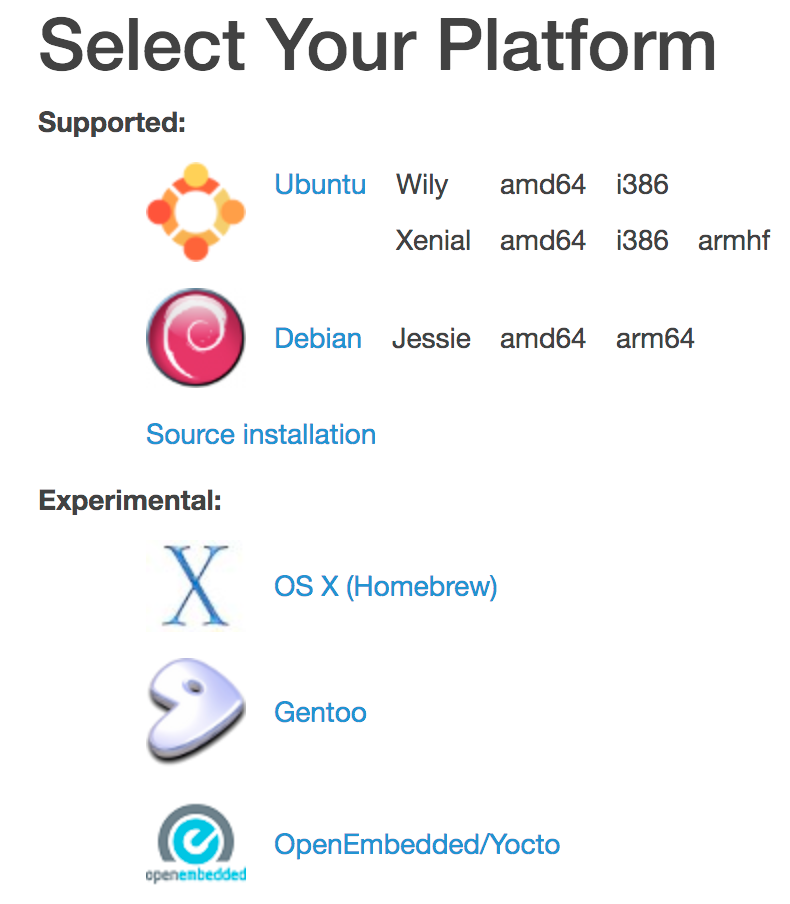
\includegraphics[width=0.5\linewidth, center]{images/Install}
  \caption{Installation choices}
  \label{fig:Installation choices}
\end{figure}

%%%%%%%%%%%%%%%%%%%%%%%%%%%%%%%%%%%%%%%%%%%%%%%%%%%%%%%%%%%%%%%%%%%%%%%%%%%%%%%%
%%%%%%%%%%%%%%%%%%%%%%%%%%%%%%%%%%%%%%%%%%%%%%%%%%%%%%%%%%%%%%%%%%%%%%%%%%%%%%%%
\clearpage
\section{METHOD}
A detailed description of what was done, how, and why; using roscore, the teleop node, installing plugins and running gazebo and rivz etc.

%%%%%%%%%%%%%%%%%%%%%%%%%%%%%%%%%%%%%%%%%%%%%%%%%%%%%%%%%%%%%%%%%%%%%%%%%%%%%%%%

\subsection{Block Diagram of running model}
%3. A block diagram of your robot setup in the ROS and Gazebo. This block diagram must show how and what messages are sent from one node to the others to make the robot move in the simulator. 

Using rosrun the run-sapce can initialise a Gazebo window. After loading up Gazebo a model can be spawned, in this case the iRobot vacuum cleaner is used. The model has been pre-edited with a plugin "differential controller" to enable control via a node "teleop node" - with the teleop node python script it is then possible to control the device. After activating a movement "rviz" is then used to capture the odometry data and produce a graphical representation of the movement with both position and direction.

\begin{figure}[H]
  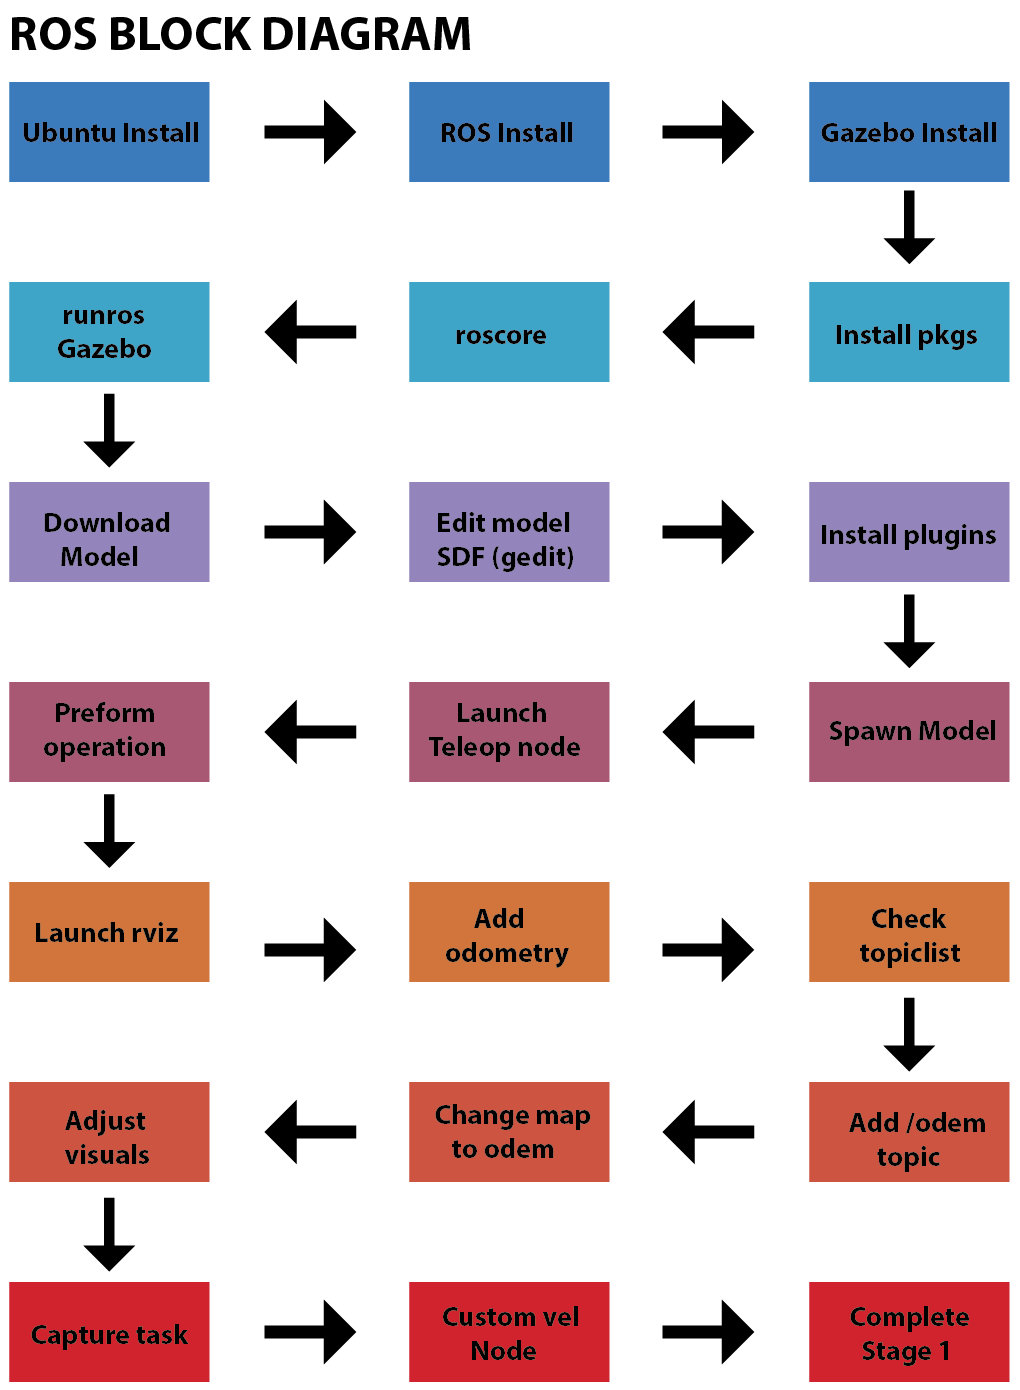
\includegraphics[width=0.8\linewidth, center]{images/Block}
  \caption{A model iRobot Create spawned in Gazebo using teleop node for movements process diagram}
  \label{fig:A model iRobot Create spawned in Gazebo using teleop node for movements process diagram}
\end{figure}

Below is a figure of the ROS and Gazebo setup showing the communication between nodes. Please note the reference from the ROS tutorials in the active diagram.

\begin{figure}[H]
  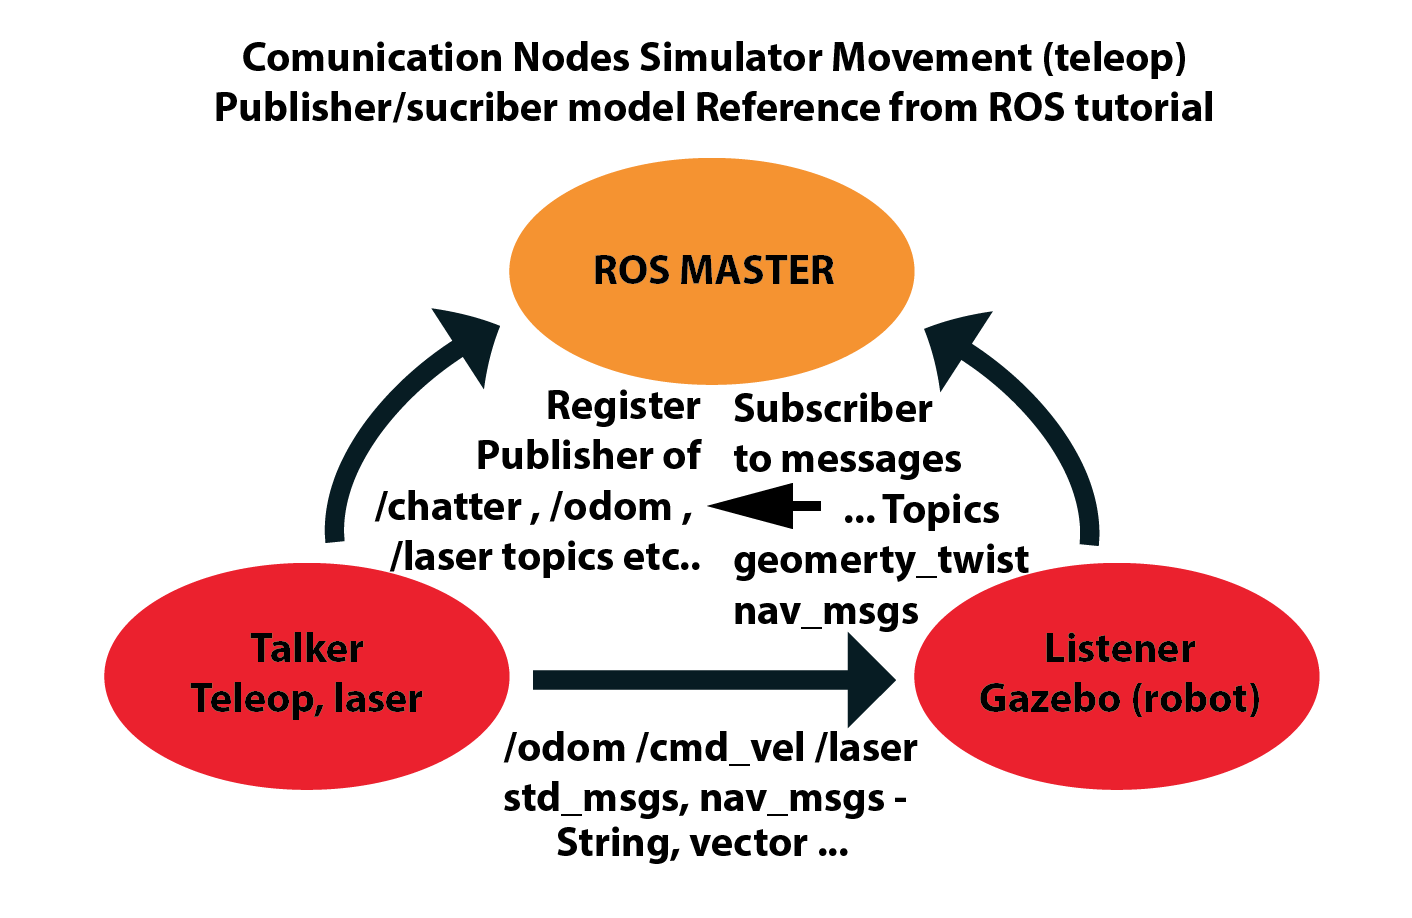
\includegraphics[width=0.8\linewidth, center]{images/BlockDiagram}
  \caption{ROS and Gazebo setup showing the communication between node}
  \label{fig:ROS and Gazebo setup showing the communication between node}
\end{figure}

Using the rqt graph command we can see that the active nodes, for this example teleop being the publisher, and gazebo the subscriber, are passed the cmd velocity; to move the differential drive for a given specific velocity and direction to describe which way for the robot to move.

\begin{figure}[H]
  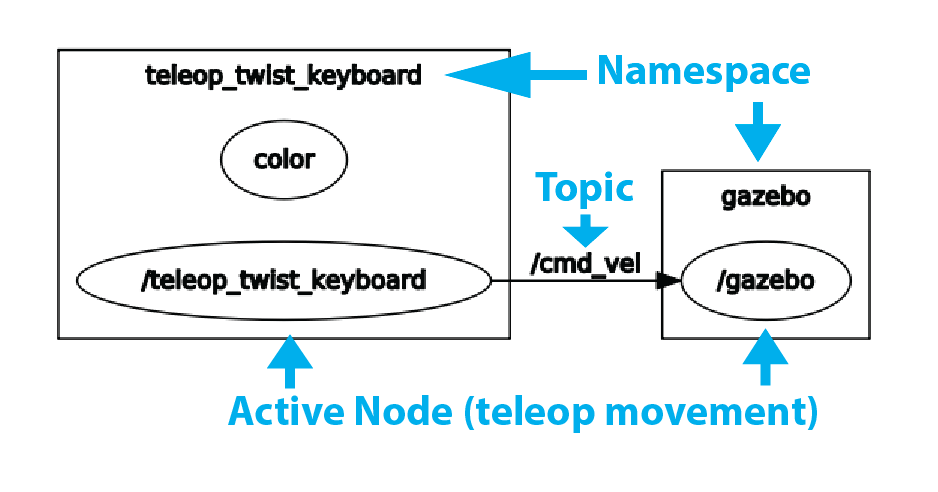
\includegraphics[width=0.8\linewidth, center]{images/rqtgraph}
  \caption{rqt graph showing active nodes}
  \label{fig:rqt graph showing active nodes}
\end{figure}

%%%%%%%%%%%%%%%%%%%%%%%%%%%%%%%%%%%%%%%%%%%%%%%%%%%%%%%%%%%%%%%%%%%%%%%%%%%%%%%%
\clearpage
\subsection{ROSCORE}
%2. Add a screenshot of ROSCORE running in a terminal 
Roscore is the fundamental processing command on which ROS can activate the simulation environment; from here gazebo can spawn models which can be edited with plugins and controlled via nodes as explained later.

\begin{figure}[H]
\begin{subfigure}{\textwidth}
	\begin{center}
  	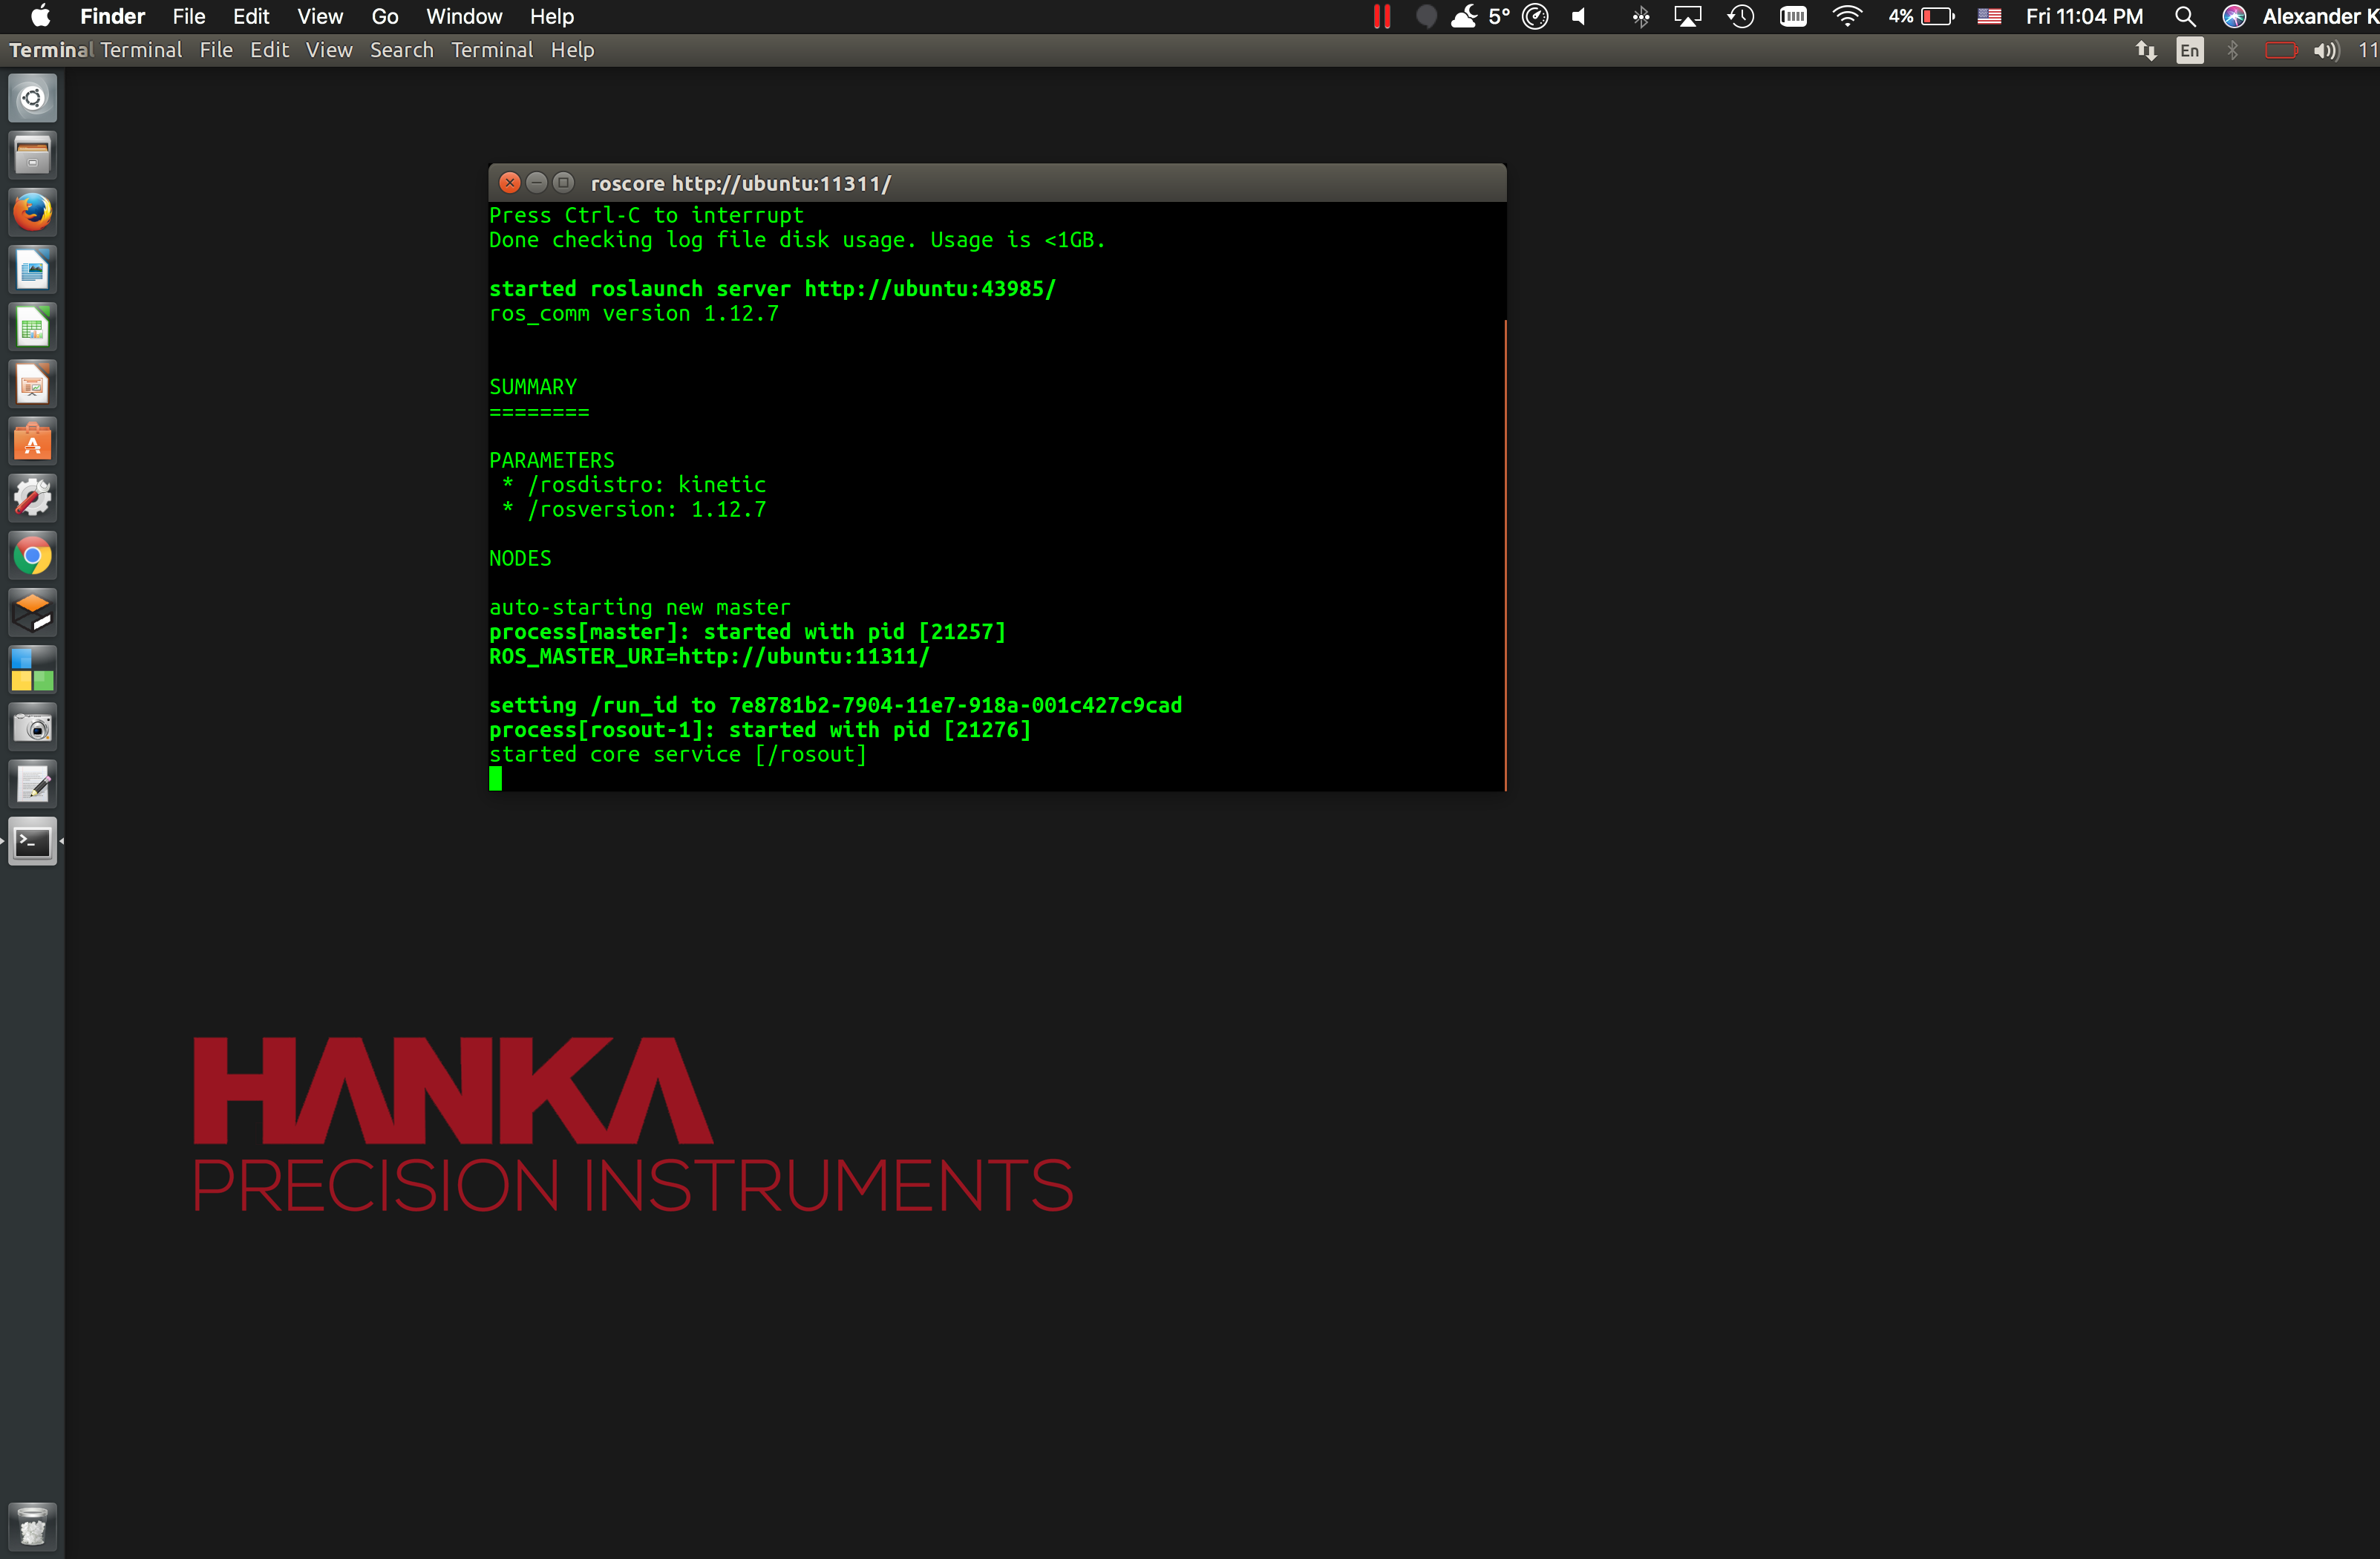
\includegraphics[width=0.7\textwidth]{images/ROSCORE}
  	\label{fig:ROSCORE running in terminal Mac Desktop}
  	\end{center}
\end{subfigure}
\begin{subfigure}{\textwidth}
	\begin{center}
  	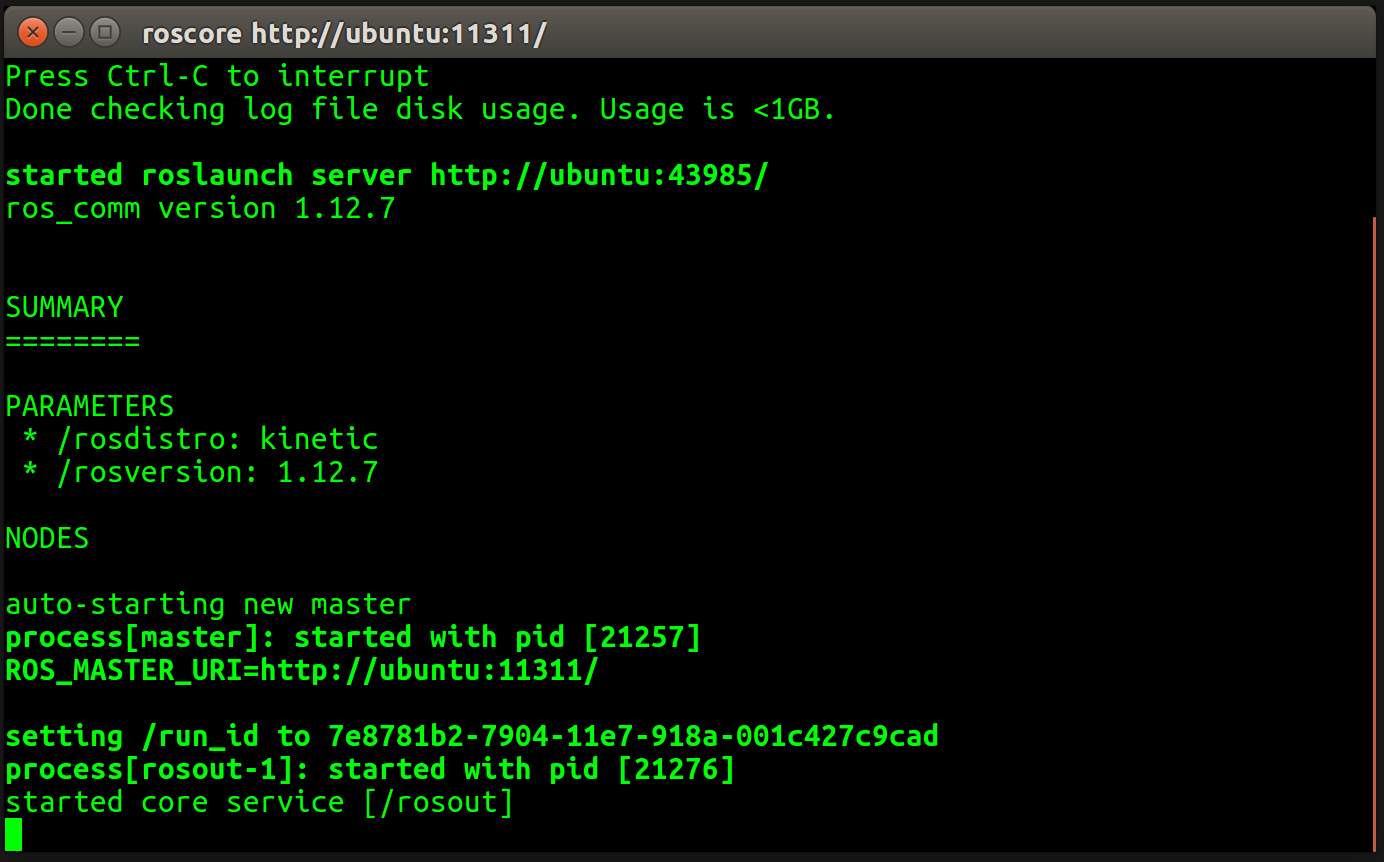
\includegraphics[width=0.7\textwidth]{images/ROSCORE2}
  	\label{fig:ROSCORE running in terminal enlarged}
  	\end{center}
\end{subfigure}
\end{figure}

Above is a demonstration of ROSCORE running in a terminal on Ubuntu operating system. This is currently in coherent mode but for better performance in later tasks the virtual runtime is switched to windowed mode.

%%%%%%%%%%%%%%%%%%%%%%%%%%%%%%%%%%%%%%%%%%%%%%%%%%%%%%%%%%%%%%%%%%%%%%%%%%%%%%%%
\clearpage
\subsection{ROS Nodes (Plugins)}
%5. What links the simulated robot in Gazebo to ROS nodes? A good explanation with figures and/or codes snippets is required.
Using some of the default plugins provided from the ROS package site, in this case the "Differential Drive" we can assign the left and right joints (wheels) to the controller. The controller in turn will take the response value passed from the Teleop Node and preform the movement in the joint.

\begin{figure}[H]
\begin{subfigure}{\textwidth}
	\begin{center}
  	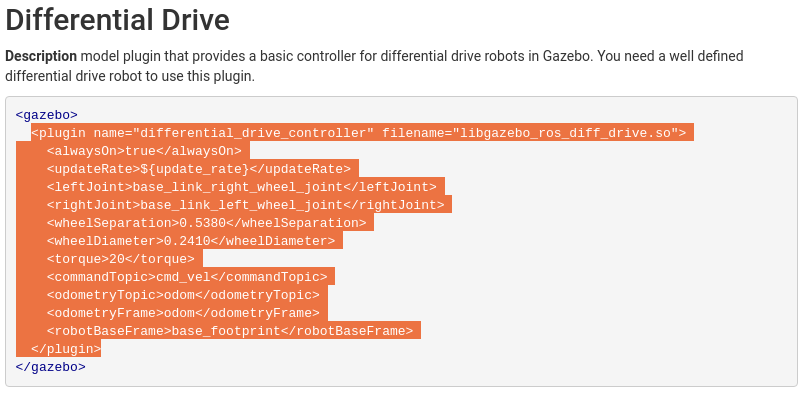
\includegraphics[width=0.7\textwidth]{images/Plugin}
  	\label{fig:Using plugins provided from ROS}
  	\end{center}
\end{subfigure}
\begin{subfigure}{\textwidth}
	\begin{center}
  	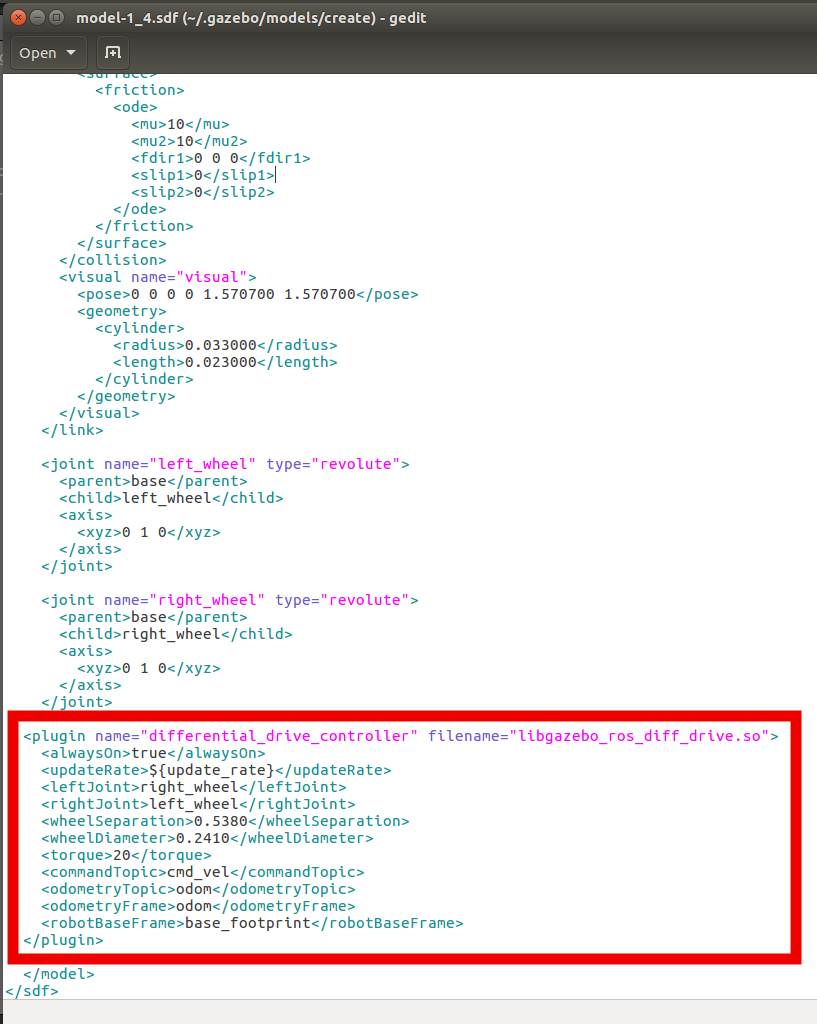
\includegraphics[width=0.7\textwidth]{images/Plugin2}
  	\label{fig:Applying the plugin}
  	\end{center}
\end{subfigure}
\end{figure}

Note: The highlighted text is copied directly without the "gazebo" tags; also once the plugin is added to the model sdf file it is then edited with gedit to match the joint name values e.g. left wheel and so on.

\clearpage
Again we can do this for the laser plugin and add the plugin to the create model 1.4

\begin{figure}[H]
  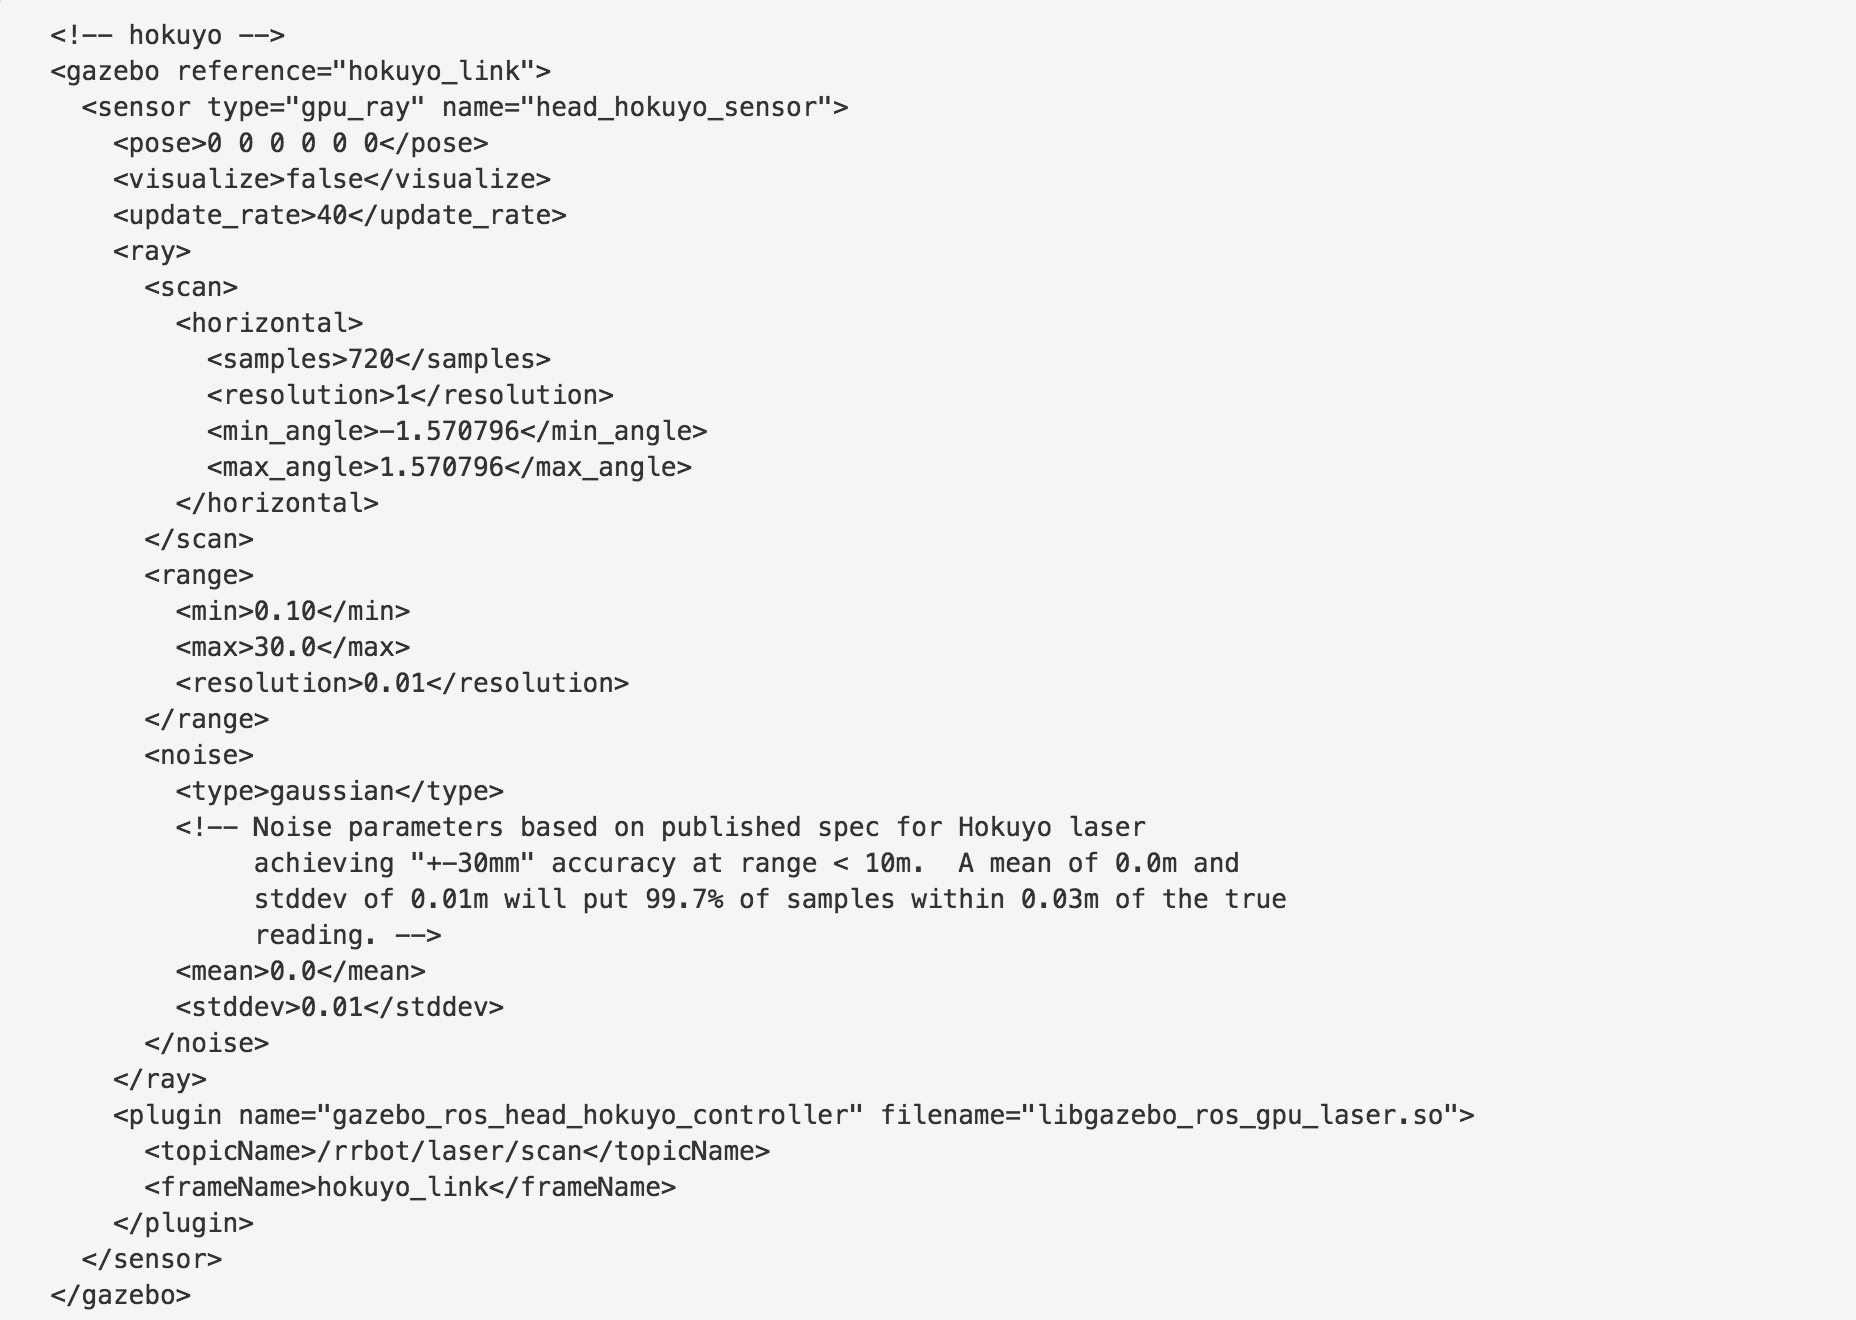
\includegraphics[width=0.8\linewidth, center]{images/laser}
  \caption{laser plugin node setup}
  \label{fig:laser plugin node setup}
\end{figure}

Here is the model with the laser scanner attached

\begin{figure}[H]
  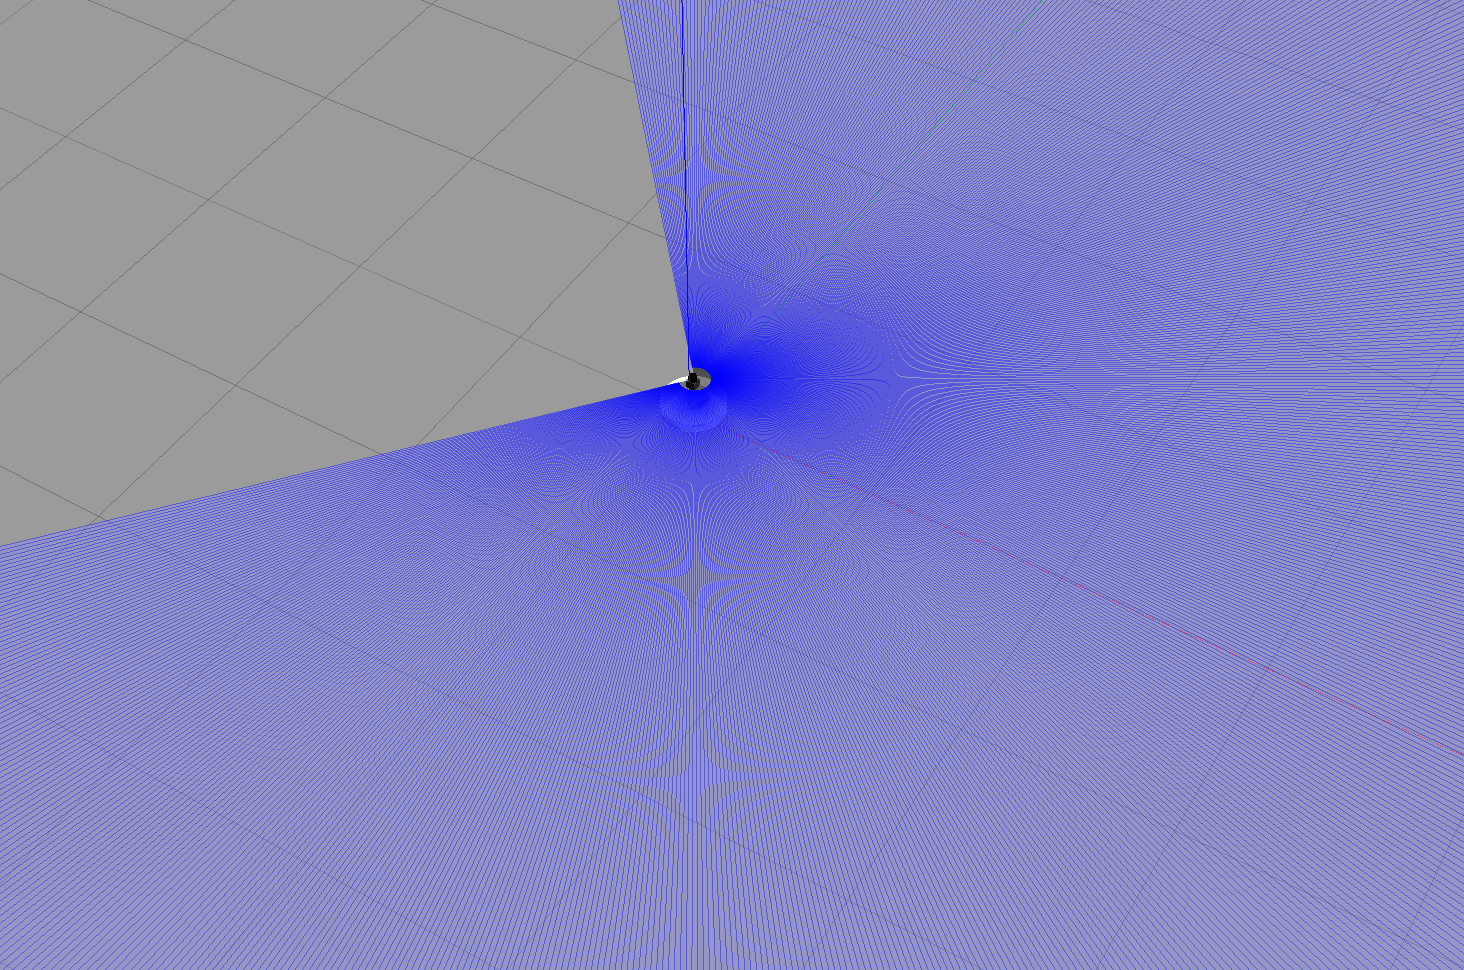
\includegraphics[width=0.8\linewidth, center]{images/laserdemo}
  \caption{laser plugin node mesh graphic}
  \label{fig:laser plugin node mesh graphic}
\end{figure}

After the plugin is assigned to the sdk file the subscriber nodes can be setup. By creating a package and compiling it, the executables can then be run and useful output given from various broadcasted topics.

\clearpage
Below is a demonstration of the odometry topic, and a node being used to give the user a notice when the 5 meter mark has bene reached in along the x and y axis. 

\begin{figure}[H]
  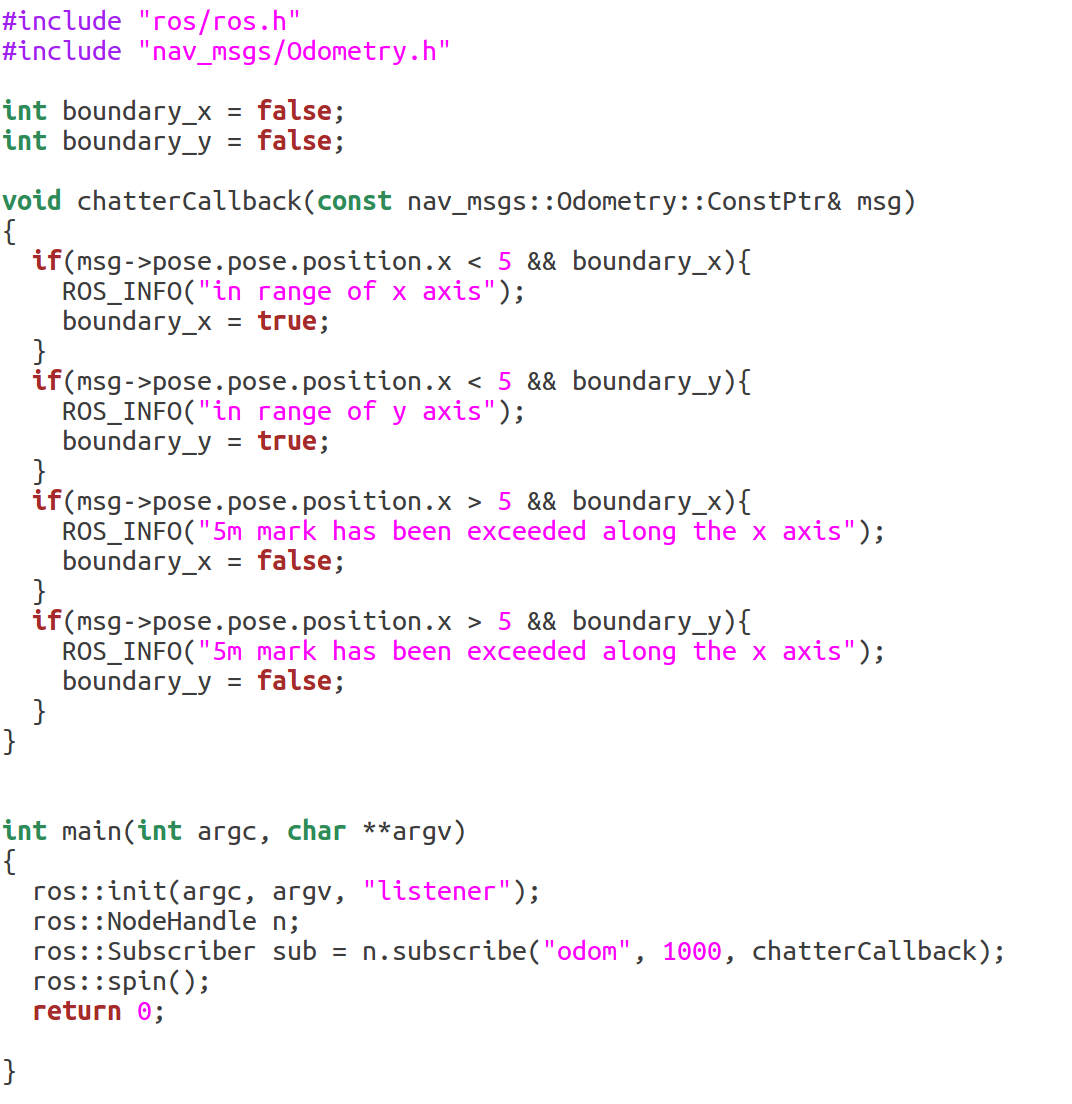
\includegraphics[width=0.8\linewidth, center]{images/odomcode}
  \caption{Subscriber odom node setup}
  \label{fig:Subscriber odom node setup}
\end{figure}

Here is the cpp code for the subscriber to the cmd velocity topic.

\begin{figure}[H]
  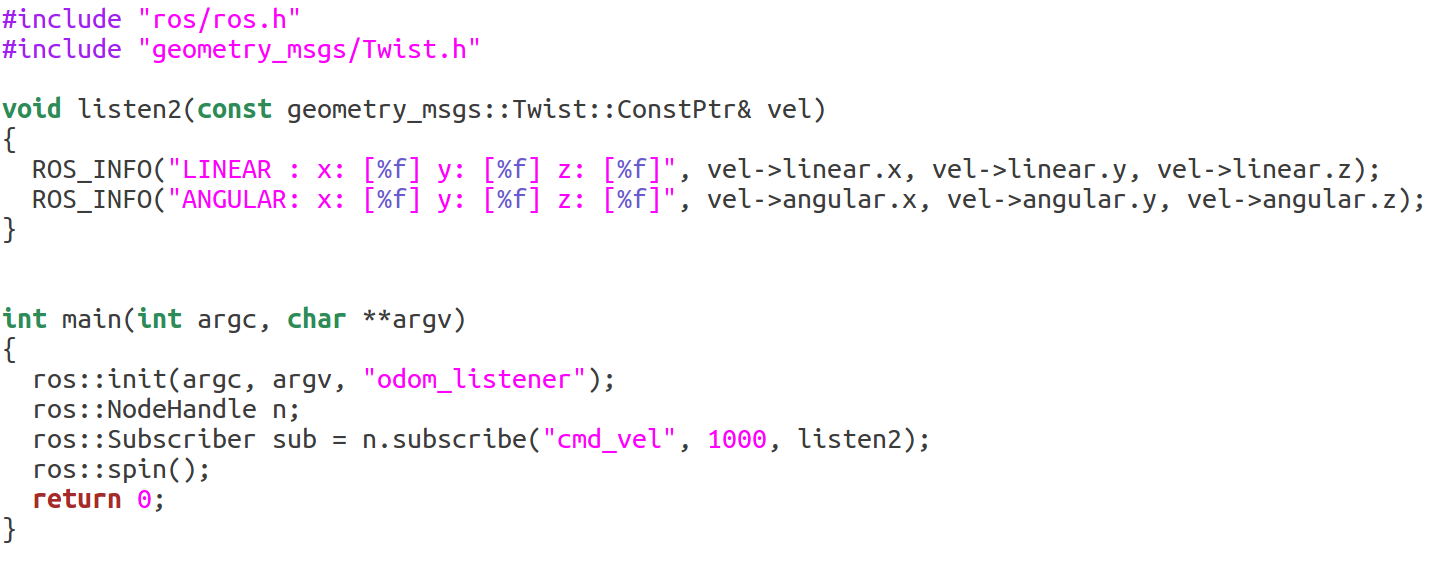
\includegraphics[width=0.8\linewidth, center]{images/cmdvelcode}
  \caption{Subscriber cmd vel node setup}
  \label{fig:Subscriber cmd vel node setup}
\end{figure}

\clearpage
Then the new cpp files are added to the cmake file to be compiled as executables the next time catkin make command is called.

\begin{figure}[H]
  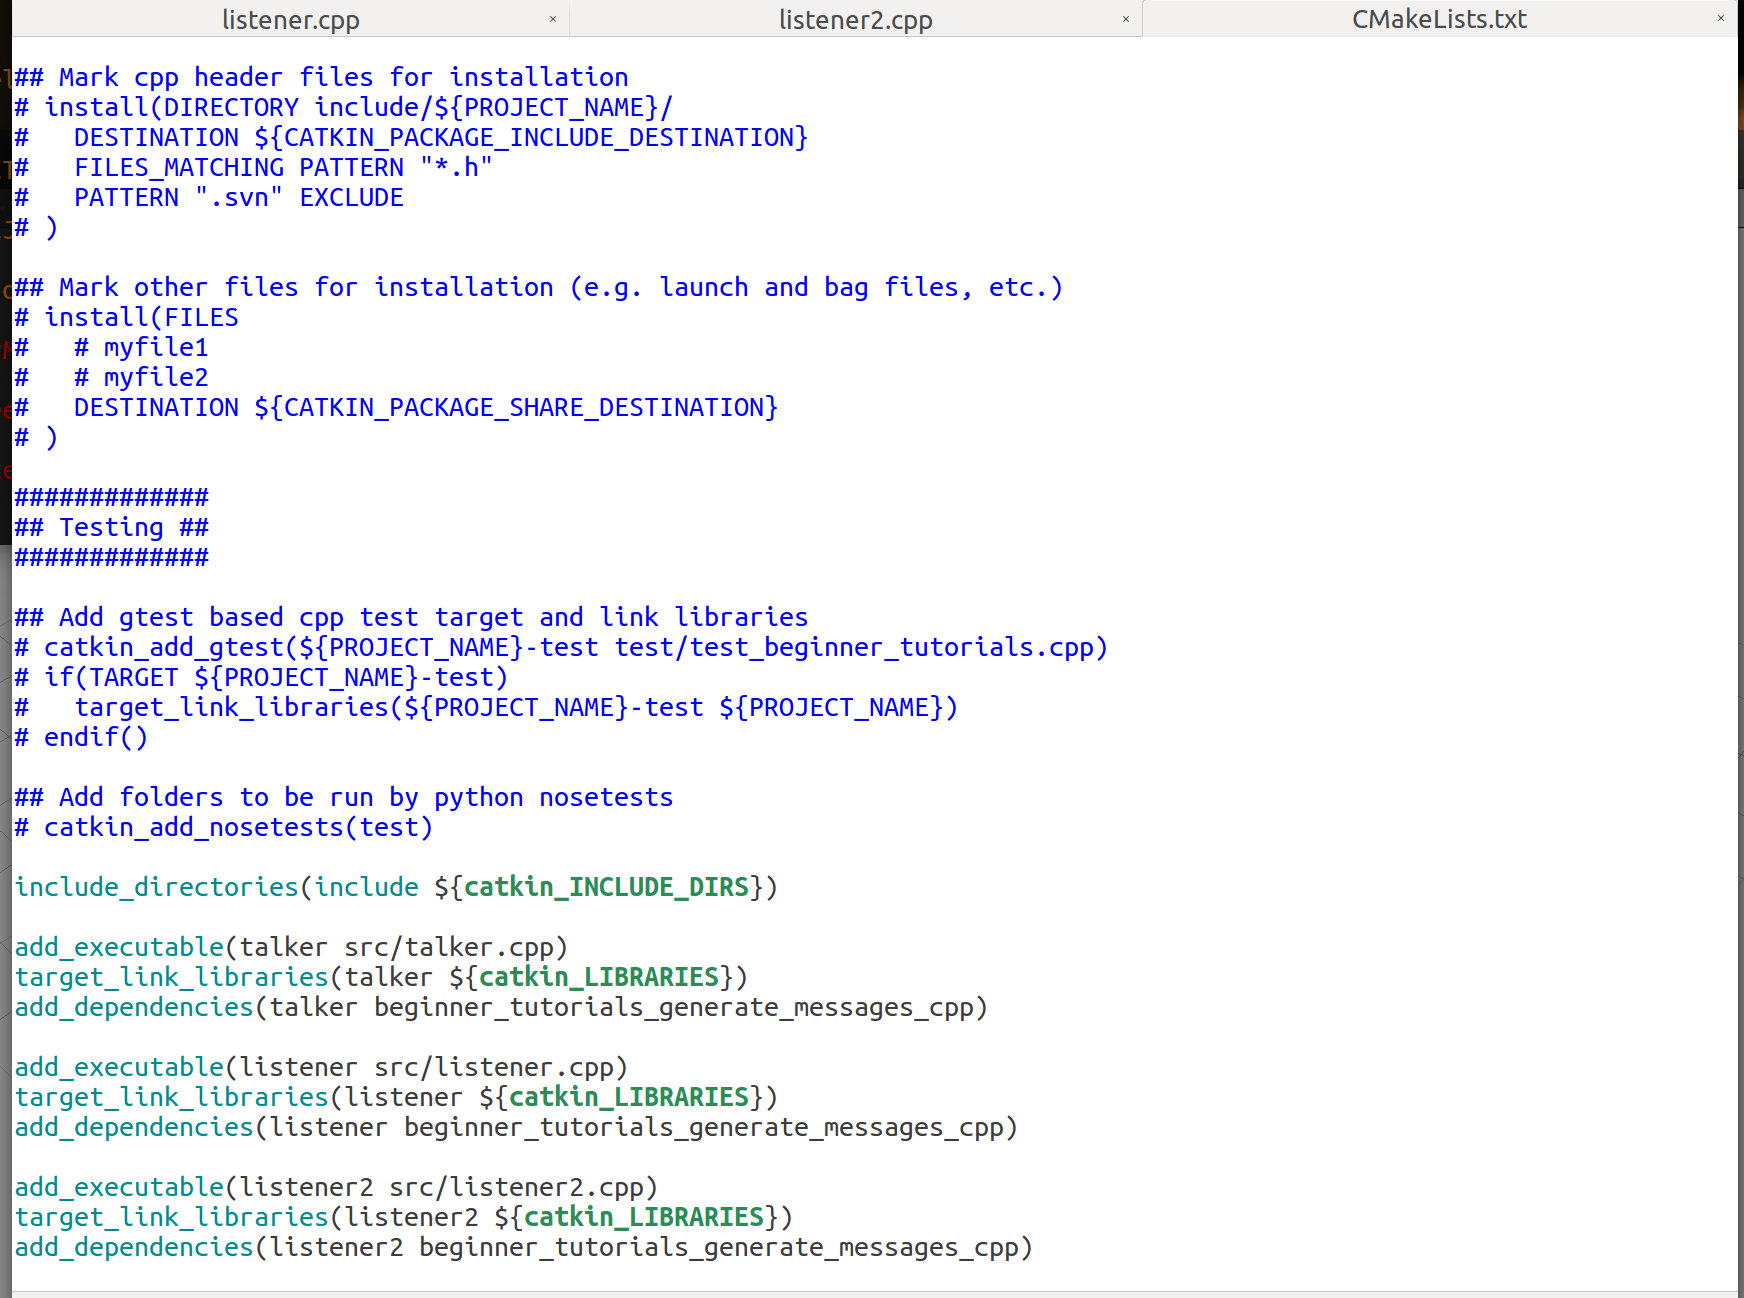
\includegraphics[width=0.8\linewidth, center]{images/exe}
  \caption{nodes executables setup}
  \label{fig:nodes executables setup}
\end{figure}

After completing and running the new node when the subscriber receives information from the broadcaster; it is then displayed on the console like the following.

\begin{figure}[H]
  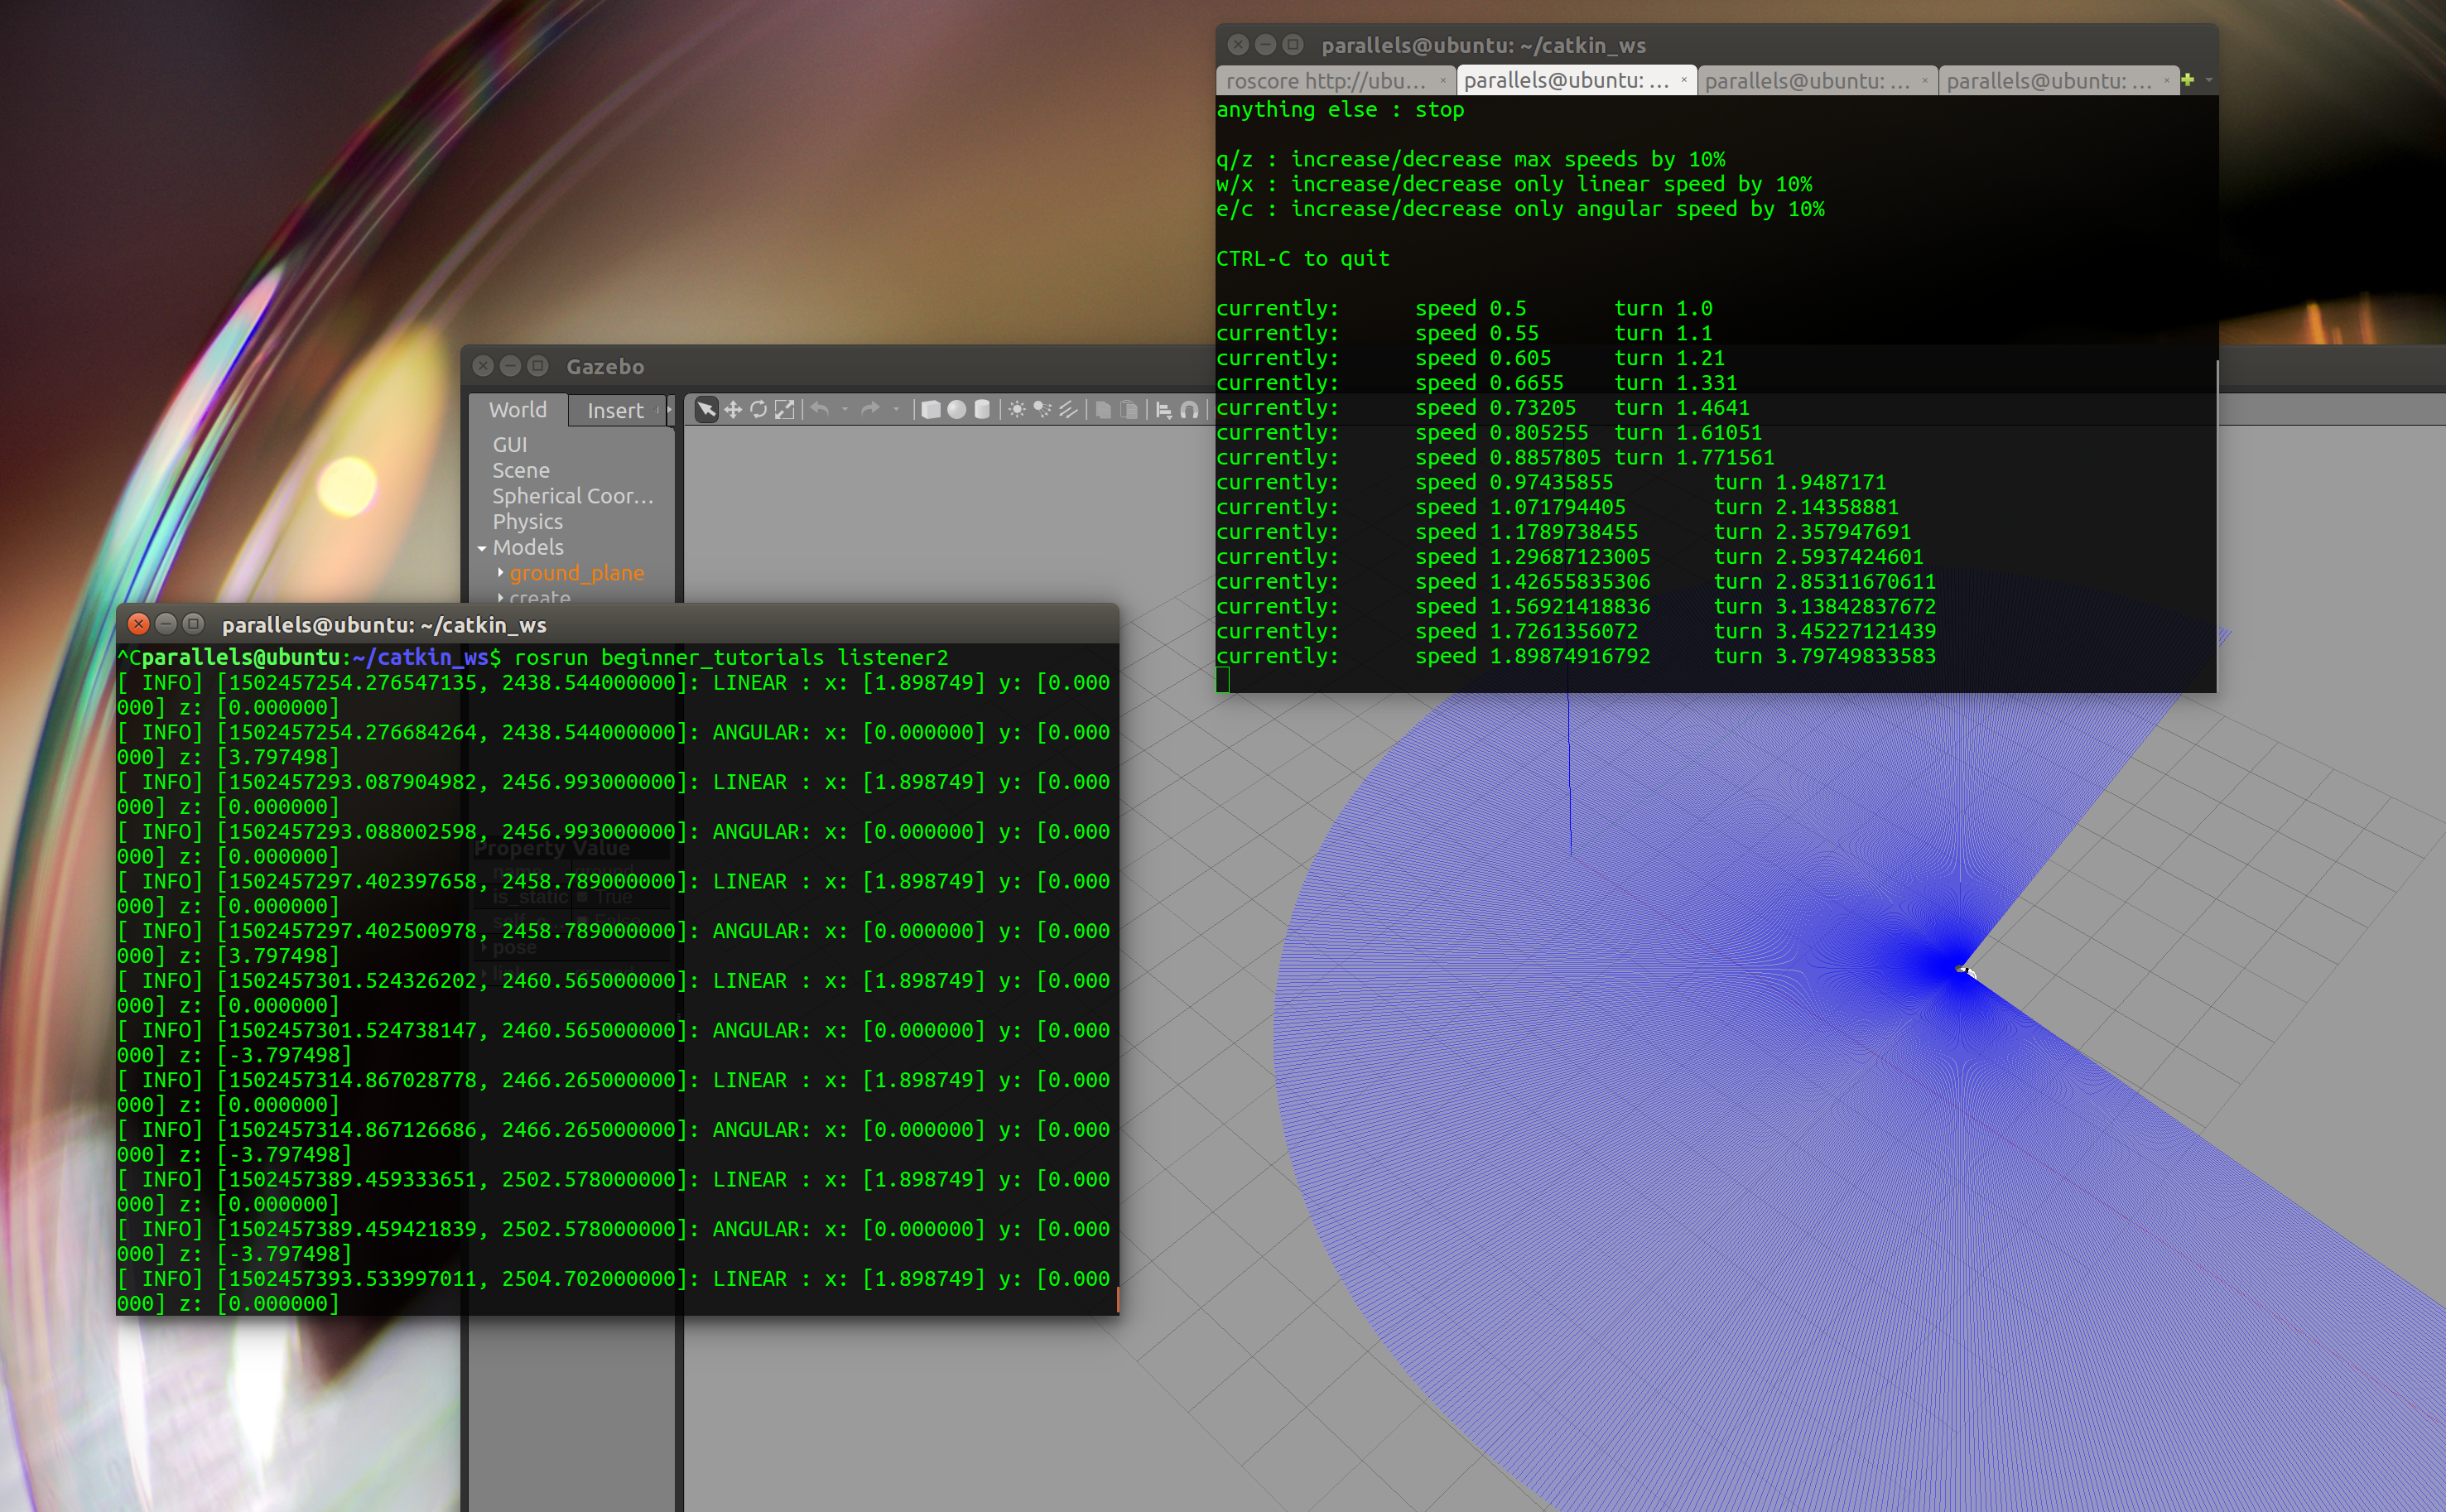
\includegraphics[width=0.8\linewidth, center]{images/cmdvelsub}
  \caption{A demo showing the cmd vel node being executed, output from the moving model}
  \label{fig:A demo showing the cmd vel node being executed, output from the moving model}
\end{figure}


%%%%%%%%%%%%%%%%%%%%%%%%%%%%%%%%%%%%%%%%%%%%%%%%%%%%%%%%%%%%%%%%%%%%%%%%%%%%%%%%
\clearpage
\subsection{Teleop Node Robot Control with Rviz}
%4. Include screenshots of "teleop node" and the robot in Gazebo at different positions. This should not be more than one page. 
Below is a demonstration of the Teleop Node used to control the left and right wheels with the plugins mentioned earlier.

\begin{figure}[H]
\begin{subfigure}{\textwidth}
	\begin{center}
  	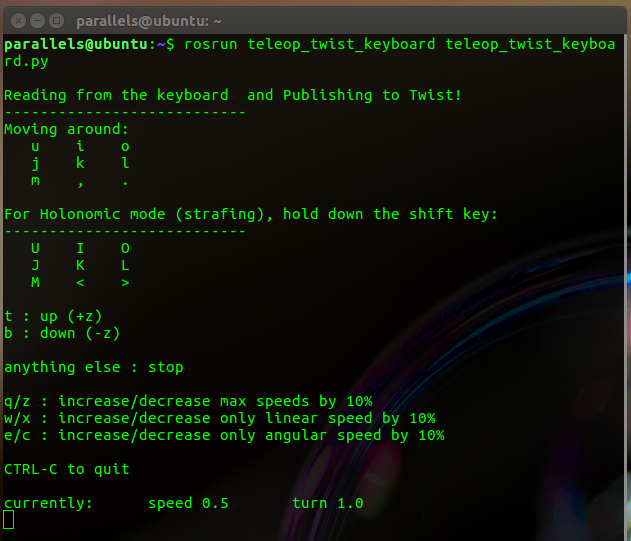
\includegraphics[width=0.7\textwidth]{images/Teleop}
  	\label{fig:Teleop node running on ubuntu}
  	\end{center}
\end{subfigure}
\begin{subfigure}{\textwidth}
	\begin{center}
  	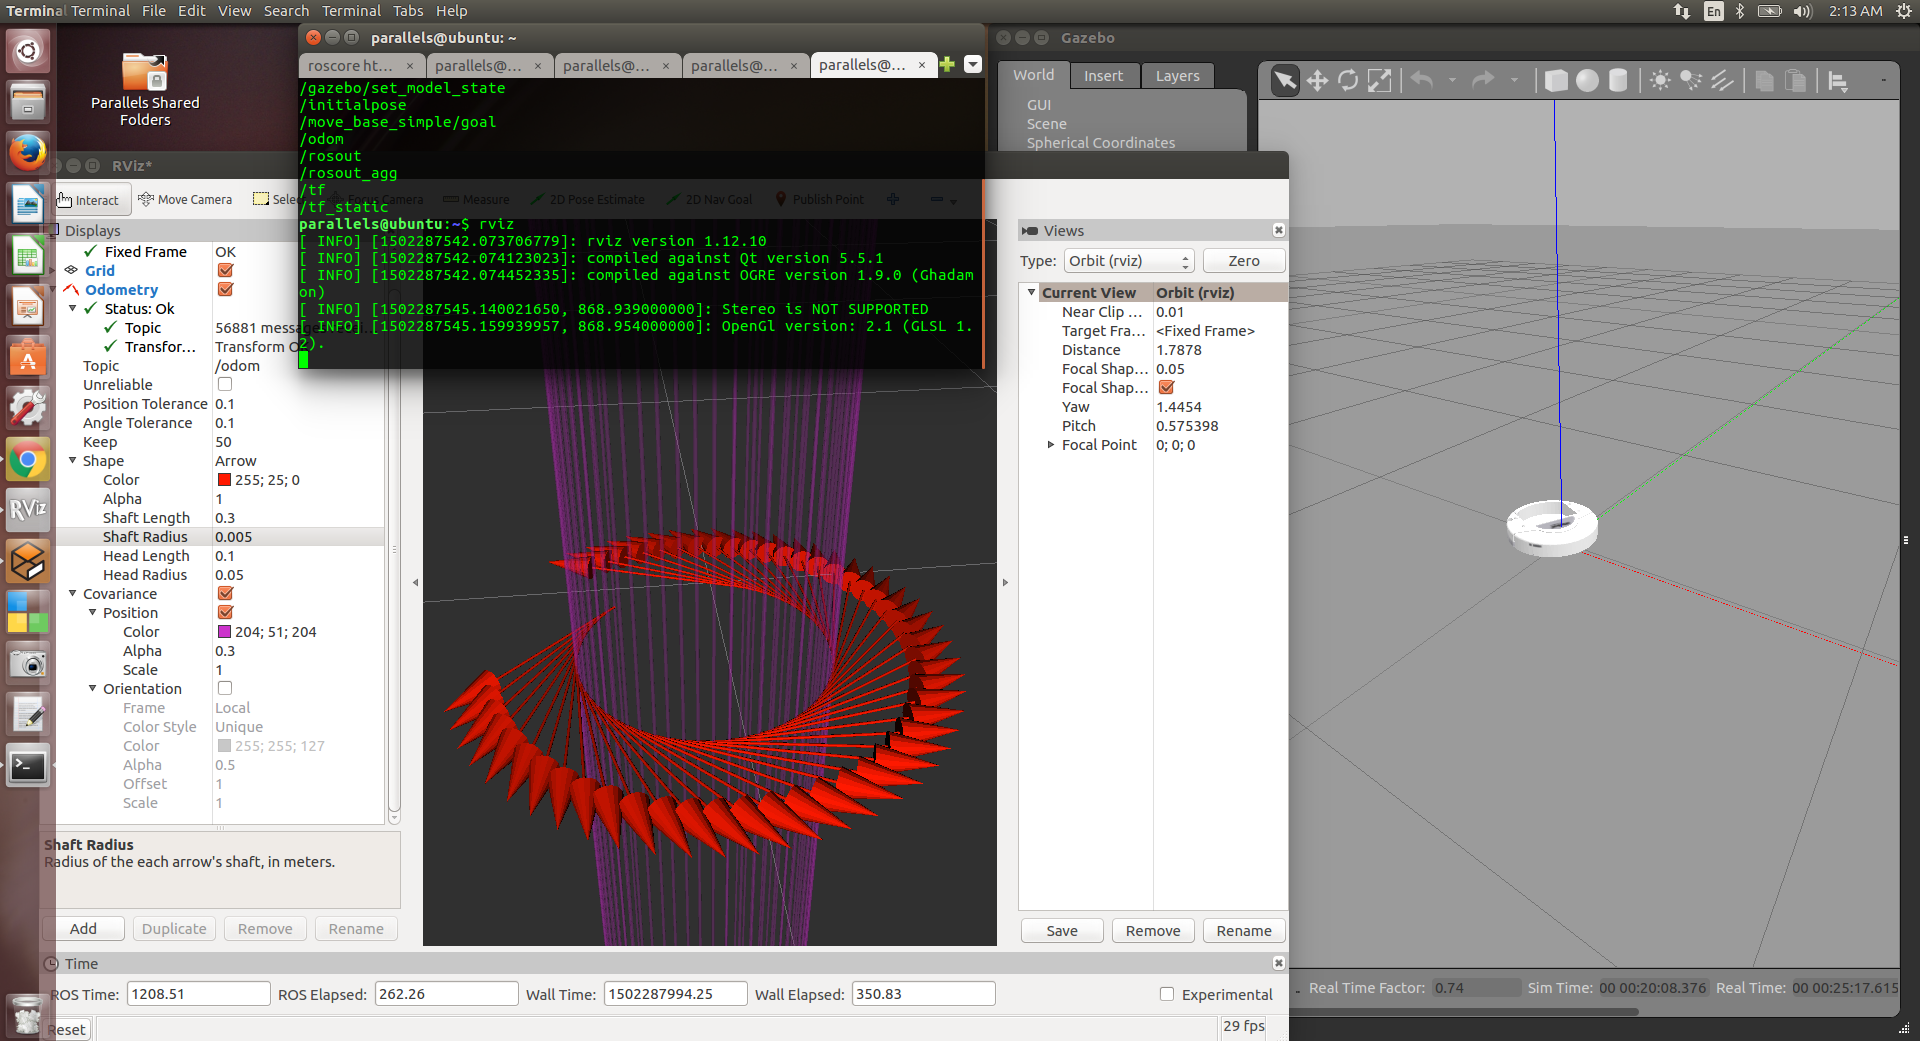
\includegraphics[width=\textwidth]{images/Position}
  	\label{fig:A model iRobot Create spawned in Gazebo using teleop node for movements}
  	\end{center}
\end{subfigure}
\end{figure}

Shown above is the rviz graphical representation of the odometry, the purple vertical lines represent the position while the red arrows show the directional vector. Rviz is great for graphical demos of what the robot interacts with in the model environment, e.g a scanner attached to find a obstacles and other objects.

\clearpage
Again Shown the rviz using the laser node with obstruction blocks and the subscribed laser topic, the representation is given by flat squares in red.

\begin{figure}[H]
  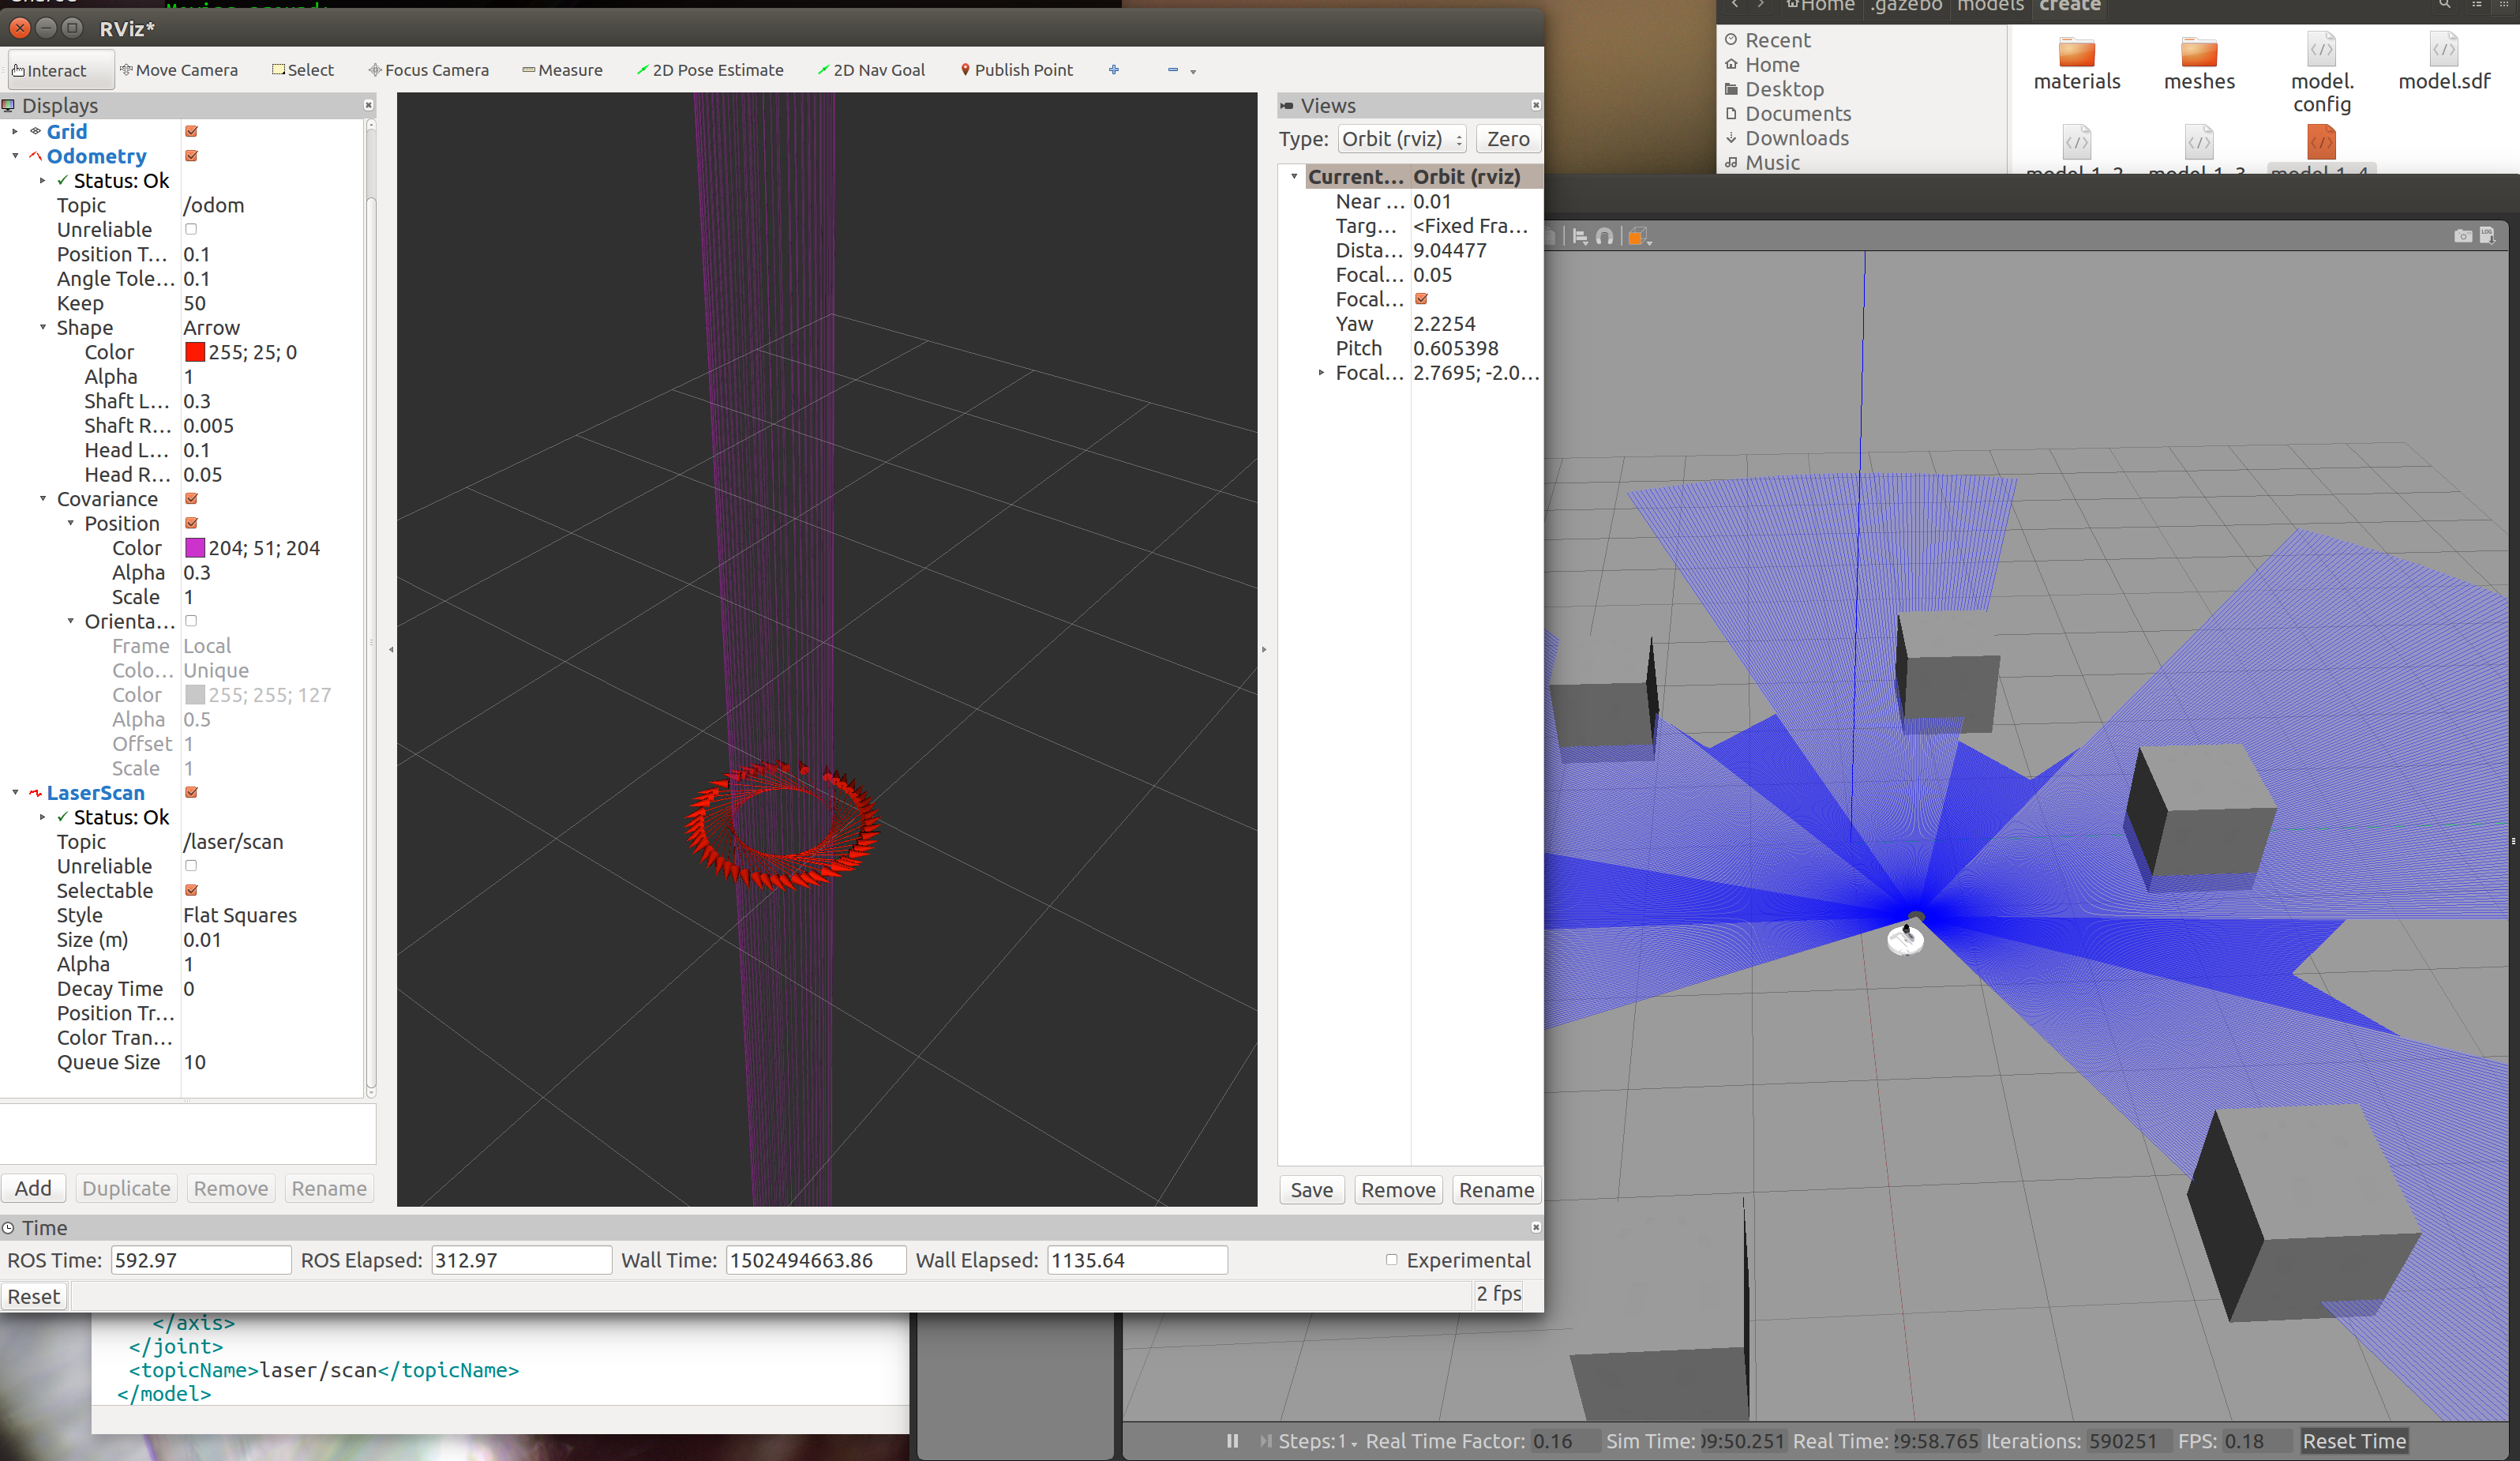
\includegraphics[width=0.8\linewidth, center]{images/rvizlaser}
  \caption{A demo showing the cmd vel node being executed, output from the moving model}
  \label{fig:A demo showing the cmd vel node being executed, output from the moving model}
\end{figure}


%7. Challenge Question: Setup "rviz" to display the topics published by the nodes. For example, the /odom, laser scan.  1

%%%%%%%%%%%%%%%%%%%%%%%%%%%%%%%%%%%%%%%%%%%%%%%%%%%%%%%%%%%%%%%%%%%%%%%%%%%%%%%%

%\subsection{Custom Node}
%6. Create a C++ node that subscribes to /cmd_vel topic advertised by Keyboard Teleop (for your selected robot) and displays1 the command in the terminal you sent to the robot. In the same node (or another) subscribe to /odom and when the robot has gone beyond a certain value of X or Y, a message is displayed in the terminal to warn the user. For example, when the robot you drive in the simulator crosses 5m along x-axis (or Euclidean distance of 5m), your node displays "going too far along x-axis" or something similar. 
 

%%%%%%%%%%%%%%%%%%%%%%%%%%%%%%%%%%%%%%%%%%%%%%%%%%%%%%%%%%%%%%%%%%%%%%%%%%%%%%%%
%%%%%%%%%%%%%%%%%%%%%%%%%%%%%%%%%%%%%%%%%%%%%%%%%%%%%%%%%%%%%%%%%%%%%%%%%%%%%%%%

%\section{RESULTS}


%%%%%%%%%%%%%%%%%%%%%%%%%%%%%%%%%%%%%%%%%%%%%%%%%%%%%%%%%%%%%%%%%%%%%%%%%%%%%%%%
%%%%%%%%%%%%%%%%%%%%%%%%%%%%%%%%%%%%%%%%%%%%%%%%%%%%%%%%%%%%%%%%%%%%%%%%%%%%%%%%

\section{OUTCOMES}

Through the above steps ROS has been successfully installed, the Gazebo runtime is used with the catkin workspace to spawn a model with edited plugins that are able to be controlled via the teleop node. 

The output is then displayed on the rviz graphical demonstration. A custom node is implemented to subscribe to the velocity topic and display the variable speed with a mentioned warning.


%%%%%%%%%%%%%%%%%%%%%%%%%%%%%%%%%%%%%%%%%%%%%%%%%%%%%%%%%%%%%%%%%%%%%%%%%%%%%%%%
%%%%%%%%%%%%%%%%%%%%%%%%%%%%%%%%%%%%%%%%%%%%%%%%%%%%%%%%%%%%%%%%%%%%%%%%%%%%%%%%

\section{CONCLUSIONS}

For any progress related to the report please see the public Github repo for alex1v1a or use the link in the cover page to be automatically redirected to this project. The repo provides all relative project information

I have come to a further understanding learned the fundamentals of ROS with the use of such simulation tools like Gazebo. I am aware of other simulation tools available but due to the community support this is a great place to start. The use of plugins with models to be controlled by the teleop python script is used in calibration with the rviz graphical output to help visualise the robots (models) sight.

This is a powerful tool and from the basic level of understanding is an extremely vital aspect of the mechatronics processing, it is a great skill to learn.

%%%%%%%%%%%%%%%%%%%%%%%%%%%%%%%%%%%%%%%%%%%%%%%%%%%%%%%%%%%%%%%%%%%%%%%%%%%%%%%%
%%%%%%%%%%%%%%%%%%%%%%%%%%%%%%%%%%%%%%%%%%%%%%%%%%%%%%%%%%%%%%%%%%%%%%%%%%%%%%%%

%\nocite{*}
%\bibliographystyle{ieeetr}
%\bibliography{references}

%%%%%%%%%%%%%%%%%%%%%%%%%%%%%%%%%%%%%%%%%%%%%%%%%%%%%%%%%%%%%%%%%%%%%%%%%%%%%%%%
%%%%%%%%%%%%%%%%%%%%%%%%%%%%%%%%%%%%%%%%%%%%%%%%%%%%%%%%%%%%%%%%%%%%%%%%%%%%%%%%

%\clearpage
%\onecolumn
%
%\section*{APPENDIX}

\end{document}
